\documentclass[11pt]{article}

\usepackage{multicol}
\usepackage{enumitem}
\usepackage{amsfonts}
\usepackage{amsmath}
\usepackage[utf8]{inputenc}
\usepackage[export]{adjustbox}  % for correct logo rendering
\usepackage{fancyhdr}  % for header/footer formatting
\usepackage{hyperref}  % for hyper-references
\usepackage{datetime}  % to update month in footer
\usepackage{array}  % more flexible tables
\usepackage[includeheadfoot,
            left=1in,
            right=1in,
            top=0.75in,
            bottom=0.75in,
            headheight=40pt]{geometry} % geometry needs to know headheight to correctly render the footer
\usepackage{tikz} % For drawing grid boxes

% desired format for footer
\newdateformat{monthyeardate}{%
  \monthname[\THEMONTH] \THEYEAR}

% set up header/footer
\pagestyle{fancy}
\fancyhf{}  % clear all headers/footers
\renewcommand{\headrulewidth}{0pt}  % remove header rule
\renewcommand{\footrulewidth}{0pt}  % remove footer rule

% set up header

\fancypagestyle{firstpage}{
    \fancyhead[L]{
    \vspace{0pt}
    \hspace{-8pt}
    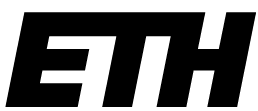
\includegraphics[width=0.1\textwidth]{docimgs/eth_logo_kurz_pos.png}\\
    \textbf{Swiss Federal Institute of Technology}\\
    \textbf{Zurich}\\
    %\textbf{ } \\
    
    }    

    \fancyhead[R]{
    \raggedleft
    %\vspace{20pt}
    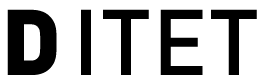
\includegraphics[width=0.13\textwidth]{docimgs/eth_ditet_logo_pos.png}\\
     \textbf{Dept. of Information Technology and} \\ \textbf{Electrical Engineering}  \\
     %\textbf{Chair for Mathematical Information} \\ \textbf{Information Science} \\

    }
}

% set up footer
\fancyfoot[L]{mdietz, linalg}
\fancyfoot[C]{\thepage}
\fancyfoot[R]{\monthyeardate\today}

% set up section/subsection titles
\renewcommand{\thesection}{\arabic{section}}
\renewcommand{\thesubsection}{\arabic{subsection}}

% command used for simply emphasizing suggestions
\newcommand{\suggestion}[1]{{\itshape #1}}


\begin{document}
\thispagestyle{firstpage}

\setlength{\headheight}{1 \baselineskip}  % accomodate header
\setlength{\parindent}{0pt}  % remove initial paragraph indent
\setlength{\parskip}{\baselineskip}  % add skip between paragraphs

%\vspace*{72px}
\vspace*{-5px}
\section*{Zusätzliche Lineare Algebra für SST1}

\section*{Themenüberblick}
\begin{itemize}
    \item \textbf{Lineare Algebra Recap:}
    \item[] Eigenwerte, Eigenvektoren, Matrixdiagonalisierung
    \item[] Normale, orthogonale, unitäre, ähnliche, und symmetrische Matrizen
    \item[] Singulärwertzerlegung
\end{itemize}

\vfill \null
\pagebreak



\setcounter{section}{1}
\renewcommand{\thesection}{1} % Custom section number

\section*{Überblick über die Grundlagen aus der Linearen Algebra für SST1}
\vspace*{-0.5cm}
\subsection*{Eigenwerte}
\vspace*{-0.5cm}
Ist $V$ ein Vektorraum und $f:V \to V$ eine Abbildung, so bezeichnet man  $v \in V$ mit $v \neq 0$ für $f(v) = \lambda v$ als Eigenvektor. Der Skalar $\lambda$ ist der dazugehörige Eigenwert.

In $\mathbb{R}^n$ (bzw $\mathbb{C}^n$): Ein Eigenwert $\lambda$ einer quadratischen Matrix $\mathbf{A}$ ist ein Skalar, für den gilt:
$$\mathbf{Ax} = \lambda \mathbf{x}$$
Um alle Eigenwerte der Matrix $\mathbf{A}$ zu finden, löst man:
$$\text{det}(\mathbf{A}-\lambda \mathbf{I}) = 0$$
Eine $n \times n$ Matrix hat mindestens einen Eigenwert und kann bis zu $n$ verschiedene Eigenwerte haben. Bei der Betrachtung von Dreiecksmatrizen sind die Eigenwerte die Elemente auf der Hauptdiagonalen. Damit ist die Determinante auch das Produkt der Eigenwerte.

Komplexe Eigenwerte einer reellen Matrix kommen als komplex konjugierte Paare vor. (i.e.: Wenn $\lambda$ ein komplexwertiger Eigenwert der reellen Matrix $\mathbf{A}$ ist, dann ist auch $\lambda^{\ast}$ ein Eigenwert von $\mathbf{A}$.)

Die \textbf{algebraische Multiplizität} eines Eigenwertes ist gleich der Ordnung der Nullstelle dieses konkreten Eigenwertes in der charakteristischen Gleichung.

Die \textbf{geometrische Multiplizität} eines bestimmten Eigenwertes entspricht der Dimension des jeweiligen Eigenraums. Es gilt immer: $1 \leq GM \leq AM$

\subsection*{Diagonalisieren einer Matrix}
\vspace*{-0.5cm}
Eine Matrix $\mathbf{A}$ ist nur dann diagonalisierbar, wenn für alle Eigenwerte gilt: GM = AM. Ist dies der Fall, so berechnet man die Eigenwerte von $\mathbf{A}$ und schreibt diese in eine Diagonalmatrix wie folgt:
$$
\mathbf{D} = \begin{bmatrix}
    \lambda_1 & & & \\
    & \lambda_2 & & \\
    & & \ddots & \\
    & & & \lambda_n
\end{bmatrix}
$$
Anschliessend berechnet man die Eigenvektoren und schreibt sie Spaltenweise in eine Matrix $\mathbf{S}$ (gleiche Reihenfolge wie die Eigenwerte):
$$\mathbf{S} = \begin{bmatrix}
    \mathbf{s}_1 & \mathbf{s}_2 & \cdots & \mathbf{s}_n
\end{bmatrix}
    $$

Damit ergibt sich die Diagonalisierung
$$\mathbf{A} = \mathbf{SDS}^{-1}$$

\pagebreak

\subsection*{Normale Matrizen}
\vspace*{-0.5cm}
Eine Matrix $\mathbf{A} \in \mathbf{R}^{n\times n}$ (bzw. $\mathbb{C}^{n \times n}$) heisst normal, falls sie $\mathbf{AA}^T = \mathbf{A}^T \mathbf{A}$ (bzw. $\mathbf{AA}^H = \mathbf{A}^H \mathbf{A}$) erfüllt.

(Komplexe) Normale Matrizen sind unitär diagonalisierbar. (Spektralsatz)

\subsection*{Orthogonale Matrizen}
\vspace*{-0.5cm}
Eine reelle quadratische Matrix $\mathbf{Q} \in \mathbb{R}^{n \times n}$ heisst orthogonal, falls
$$\mathbf{Q}^T \mathbf{Q}= \mathbf{I} \Leftrightarrow \mathbf{Q}^{-1} = \mathbf{Q}^T$$
Diese Bedingung ist gleichbedeutend mit $$\mathbf{q}_i^T \cdot \mathbf{q}_j = \delta_{ij} = \begin{cases}
    1, & i = j \\
    0, & i \neq j
\end{cases}$$
wobei $\mathbf{q}_i$ die Spaltenvektoren von $\mathbf{Q}$ sind und $\delta_{ij}$ das Kronecker delta bezeichnet.

Die Spaltenvektoren einer orthogonalen Matrix bilden somit eine Orthonormalbasis des Koordinatenraums $\mathbb{R}^n$. Dies gilt auch für die Zeilenvektoren, denn wenn $\mathbf{Q}$ orthogonal ist, so ist auch $\mathbf{Q}^T$ orthogonal.

Für Orthogonalität reicht nicht aus, dass die Spaltenvektoren paarweise orthogonal sind. Die Spaltenvektoren müssen zusätzlich auch normiert sein.

Orthogonale Matrizen sind längen- und winkeltreu, d.h.:
$$||\mathbf{Qx}||_2 = ||\mathbf{x}||_2, \hspace{20pt} \langle \mathbf{Qx}, \mathbf{Qy} \rangle = \langle \mathbf{x}, \mathbf{y}\rangle$$

Der Betrag der Determinante einer orthogonalen Matrix ist stets 1. ($|\text{det}\mathbf{Q}| = 1$)

Die Eigenwerte einer orthogonalen Matrix sind nicht notwendigerweise alle reell, haben jedoch stets den Betrag 1 und sind somit von der Form: $\lambda = e^{i\theta}, \; \theta \in \mathbb{R}$

Orthogonale Matrizen sind normal, da $\mathbf{QQ}^T = \mathbf{Q}^T \mathbf{Q}$ und somit unitär diagonalisierbar. (Spektralsatz)

\subsection*{Unitäre Matrizen}
\vspace*{-0.5cm}
Eine Unitäre Matrix ist eine Matrix, bei welcher gilt:
$$\mathbf{Q}^H \mathbf{Q} = I \Leftrightarrow \mathbf{Q}^H = \mathbf{Q}^{-1}$$
(Dieses Konzept ist das komplexe Analogon zu Orthogonalität.)

\subsection*{Ähnliche Matrizen}
\vspace*{-0.5cm}
Zwei Matrizen $\mathbf{A}$ und $\mathbf{B}$ sind ähnlich, falls eine invertierbare Matrix $\mathbf{S}$ existiert, sodass
$$\mathbf{A} = \mathbf{S}^{-1} \mathbf{BS}$$
Im Fall einer Diagonalisierung ist also die Matrix $\mathbf{A}$ ähnlich zu ihrer Diagonalmatrix $\mathbf{D}$. Ähnliche Matrizen haben die gleichen Eigenwerte und somit das gleiche charakteristische Polynom.

\subsection*{Symmetrische Matrizen}
\vspace*{-0.5cm}
Falls, $\mathbf{A} = \mathbf{A}^T$, so ist $\mathbf{A}$ eine symmetrische Matrix. (Analog: Falls $\mathbf{A}$ komplexwertig ist und $\mathbf{A} = \mathbf{A}^H$, so ist $\mathbf{A}$ hermite-symmetrisch)

Symmetrische Matrizen sind normal, denn es gilt trivialerweise $\mathbf{AA}^T = \mathbf{A}^T \mathbf{A}$

Symmetrische Matrizen haben stets relle Eigenwerte und paarweise orthogonale Eigenvektoren.

Jede symmetrische Matrix lässt sich durch orthogonale Transformationen diagonalisieren.
$$\mathbf{A} = \mathbf{UDU}^{-1} = \mathbf{UDU}^T$$

\subsection*{Singulärwertzerlegung}
\vspace*{-0.5cm}
Die SVD zerlegt eine beliebige Matrix $\mathbf{A} \in \mathbb{R}^{m\times n}$ in zwei orthogonale Matrizen $\mathbf{U} \in \mathbb{R}^{m\times m}$ und $\mathbf{V} \in \mathbf{R}^{n\times n}$ und eine Matrix $\mathbf{\Sigma} \in \mathbb{R}^{m \times n}$ mit den Singulärwerten auf der Hauptdiagonalen.
$$\mathbf{A} = \mathbf{U\Sigma V}^T = \begin{bmatrix}
    \mathbf{U}_r & \mathbf{U}_k
\end{bmatrix} \begin{bmatrix}
    \mathbf{\Sigma}_r & \mathbf{0} \\
    \mathbf{0} & \mathbf{0}
\end{bmatrix} \begin{bmatrix}
    \mathbf{V}_r^T \\
    \mathbf{V}_k^T
\end{bmatrix}$$
Es ist dabei $\mathbf{\Sigma} = \text{diag}(\sigma_1, \sigma_2, \dots,\sigma_r )$. Diese Werte sind absteigend sortiert.

Gegeben eine SVD einer Matrix $\mathbf{A}$, so gilt:
\vspace*{-0.5cm}
\begin{itemize}
    \item Rang($\mathbf{A}$) = Anzahl Singulärwerte $>$ 0
    \item $\text{dim}(\mathbf{A}) = \text{dim}(\mathbf{\Sigma})$
    \item ONB von Bild($\mathbf{A}$) = $\text{span}\{u_1, \dots, u_r\}$
    \item ONB von Kern($\mathbf{A}$) = $\text{span}\{v_{r+1}, \dots, v_n\}$
\end{itemize}

\end{document}
